\chapter{Modelado conceptual, diagramas entidad/relación}

\section{Etapas de la creación de una BD}

Una base de datos es una representación informática de un sistema real, por lo que deben seguirse una serie de pasos en su proceso de creación para garantizar que ésta sea fiel a aquello que se quiere representar y gestione dichos de forma eficiente:

\begin{itemize}
	\item\textbf{Obtención de datos generales:} Mediante una entrevista con el cliente, se obtienen datos sobre la organiazción para la cual se va a crear la BD\@. Estos datos ofrecen una imagen amplia del sistema necesaria para juzgar qué decisiones de diseño deberemos tomar.
	\item\textbf{Extracción de datos operativos:} A lo largo de la entrevista se mencionan datos cuantificables y plasmables como enunciado de un problema. Éstos son los datos con los que trabajamos en la BD\@.
	\item\textbf{Creación de un esquema conceptual de la BD:} Una vez obtenidos los datos operativos creamos un diagrama de relación entre ellos asignándoles a cada uno un tipo de dato. De esta clasificación se obtiene el esquema conceptual de la BD\@.
	\item\textbf{Creación de un modelo lógico de la BD:} Con los datos clasificados por tipo implementamos un modelo con estructuras de datos. A lo largo de estas prácticas nos centraremos en el modelo relacional, cuya estructura está formada por tablas.
	\item\textbf{Implementación de la BD en un SGBD:} Creada la BD, la implementamos en un SGBD para trabajar con ella a alto nivel.
\end{itemize}

\section{El modelo E/R}

El modelo E/R es un mecanismo formal para representar y manipular información de manera general y sistemática.
Este modelo, al igual que otros, sigue una serie de claves para su uso:

\begin{itemize}
	\item\textbf{Datos:} Son un recurso de gran importancia para la empresa contratante de la BD, ya que su control supone una ventaja para ella. Deben ser analizados con detenimiento.
	\item\textbf{Convenciones:} Se aplica una notación rigurosa y normalizada y se sigue una línea de actuación sistemática, garantizando una ambigüedad nula en la lectura del modelo.
	\item\textbf{Redundancia mínima:} Idualmente, cada dato o concepto debe ser modelado una única vez y de una única formal.
\end{itemize}

El modelado E/S es la técnica de diseño conceptural más extendida, ya que posee una gran capacidad extensiva, rigurosidad en la forma, simplicidad de diseño y facilidad de uso.
Todo esto se consigue gracias a principios de diseño que garantizan cercanía entre la representación y los datos representados, calidad en dicha representación y facilidad de transmisión del modelo.
Este modelo debe reflejar las necesidades de información de una organización, ya que será usado como base para el desarrollo de un sistema, y ofrecer un diseño independiente del posterior almacenamiento y métodos de acceso a los datos, permitiendo así tomar decisiones objetivas y sin restricciones sobre la mejor implementación de la BD\@.

El modelo E/R ofrece las siguientes características:

\begin{itemize}
	\item\textbf{Independencia de etapas posteriores:} Se ignoran el modelo de datos para el esquema lógico, el SGBD y el modo de almacenamiento y acceso a los datos que se usarán en el futuro.
	\item\textbf{Jerarquización de los datos:} Es el diseñador quien decide qué datos son más relevantes que los demás, evitando ruido en el modelo por exceso de datos o falta de funcionalidad del sistema por falta de los mismo.
	\item\textbf{Restricciones en la especificación:} El modelo se elabora a partir de ellos, ofreciendo rigurosidad y uniformidad en el producto final.
	\item\textbf{Rapidez y agilidad en el modelado.}
\end{itemize}

\section{Elementos básicos de modelo}

\subsection{Entidades}

Los atributos son objetos de nuestro interés agrupados por tipos.
Estos objetos existen en el sistema que estamos representando mediante la BD y son distinguibles entre sí.
Por ejemplo, en una BD de una biblioteca podríamos tener $personal$, $libros$ y $revistas$ como tipos de entidades y diferentes entidades de $libros$ individuales.

Las entidades pueden depender existencialmente de otras:

\begin{displayquote}
Sean $A$ y $B$ dos conjuntos de entidades, decimos que $B$ depende existencialmente de $A$ si se cumple:

\begin{itemize}
	\item$\exists T\in A\times B/\forall b\in B \Rightarrow\exists a\in A/(a,b)\in T,y$.
	\item Es imposible identificar a $b$ sin identificar previamente a $a$.
\end{itemize}
\end{displayquote}

Esta dependencia se produce cuando la existencia de cada entidad $b\in B$ está condicionada por la existencia de una entidad $a\in A$ para dos conjuntos $A$ y $B$.
Decimos que una entidad es débil si depende existencialmente de otra, que es fuerte.
Por ejemplo, una $cuenta\ bancaria$ es una entidad débil, pues depende existencialmente de su $titular$.

En un sistema puede existir más de una entidad débil que dependa de una misma entidad fuerte, en cuyo caso siembre debe haber un atributo discriminador que permita diferenciar cada una de dichas entidades débiles.

\subsection{Atributos}

Los atributos son las propiedades por las que se caracteriza un conjunto de entidades.
Por ejemplo, podrían ser atributos de una \code{Criatura} su \code{Fuerza}, \code{Defensa}, \code{Habilidades} y \code{Coste}.

Cuando trabajamos con atributos debemos tener en cuenta su \textbf{dominio}, que el conjunto de valores permitidos que puede tomar cada uno.
Por ejemplo, el dominio de la fecha de creación de una cuenta en una red social se compone por todos los días desde la creación de ésta hasta la actualidad, actualizándose diariamente para permitir cuentas nuevas.

Cuando podemos identificar unívocamente a una entidad mediante un atributo o un conjunto de éstos decimos que éstos son su \textbf{clave candidata o primaria}.
Por ejemplo, cada ciudadano español tiene su propio NIF y cada usuario de GitHub se identifica por su nombre de usuario.

\subsection{Relaciones}

Las relaciones o asociaciones son conexiones semánticas entre dos o más conjuntos de entidades.

La \textbf{cardinalidad} de una relación es el número máximo de entidades de un conjunto que se relacionan con una entidad de otro y viceversa.
Cuando las relaciones son binarias (entre dos entidades) distinguimos entre tres cardinalidades:

\begin{itemize}
	\item\textbf{Uno a uno (\code{1:1}):} Cada instancia de una entidad se relaciona con una única instancia de otra y viceversa. \textit{Un libro tiene un ISBN}.
	\item\textbf{Uno a muchos (\code{1:m}):} Cada instancia de una entidad se relaciona con varias instancias de otra pero las instancias de la segunda entidad se relacionan con una única instancia de la primera. \textit{Una fábrica emplea varios trabajadores}.
	\item\textbf{Muchos a muchos (\code{n:m}):} Cada instancia de una entidad se relaciona con varias de otra y viceversa. \textit{Muchos lectores leen muchos apuntes}.
\end{itemize}

Debemos tener en cuenta que esta cardinalida depende de la implementación de la BD\@.
Por ejemplo, \textit{una fábrica emplea varios trabajadores} podría no ser un relación \code{1:m} si tuviéramos un sistema en el que controláramos varias fábricas y algunos de los operarios estuvieran pluriempleados (en este caso sería \code{n:m}) pero sí lo sería si estuviéramos trabajando únicamente con los datos internos de la fábrica en cuestión.

Las relaciones también pueden tener atributos discriminadores y característicos.
Por ejemplo, cuando un \textit{cliente combra un producto} lo hace en una \textit{fecha y hora} determinadas y compra una \textit{cantidad} de dicho producto.

Decimos que una relación es \textbf{involutiva} cuando conecta un conjunto de entidades consigo mismo.
Formalmente la expresamos de la siguiente manera:

\[T\subseteq A\times B\text{ es involutiva}\Leftrightarrow B=A\]

En este caso, debemos asignar una etiqueta o rol a cada participación de la entidad $A$ en $T$.
Por ejemplo, si tenemos la relación \textit{persona paga a persona} una de ellas debe ser la persona \textit{emisora} del dinero y la otra, la \textit{receptora}.

\section{Diagramas E/R}

El modelo E/R se basa en la realización de diagramas, ya que estos permiten plasmar la información que queremos gestionar en la base de datos de forma ordenada y son un medio sencillo y fácilmente comprensible para especificar el diseño conceptual.
La característica más importante es que estos diagramas son idependientes del modelo con el que posteriormente se implemente la BD\@.

En este modelo representamos las entidades como rectángulos y las relaciones entre ellas como rombos.
Las entidades débiles se representan como rectángulos de doble perfilado.

\begin{figure}[h]
\begin{center}
	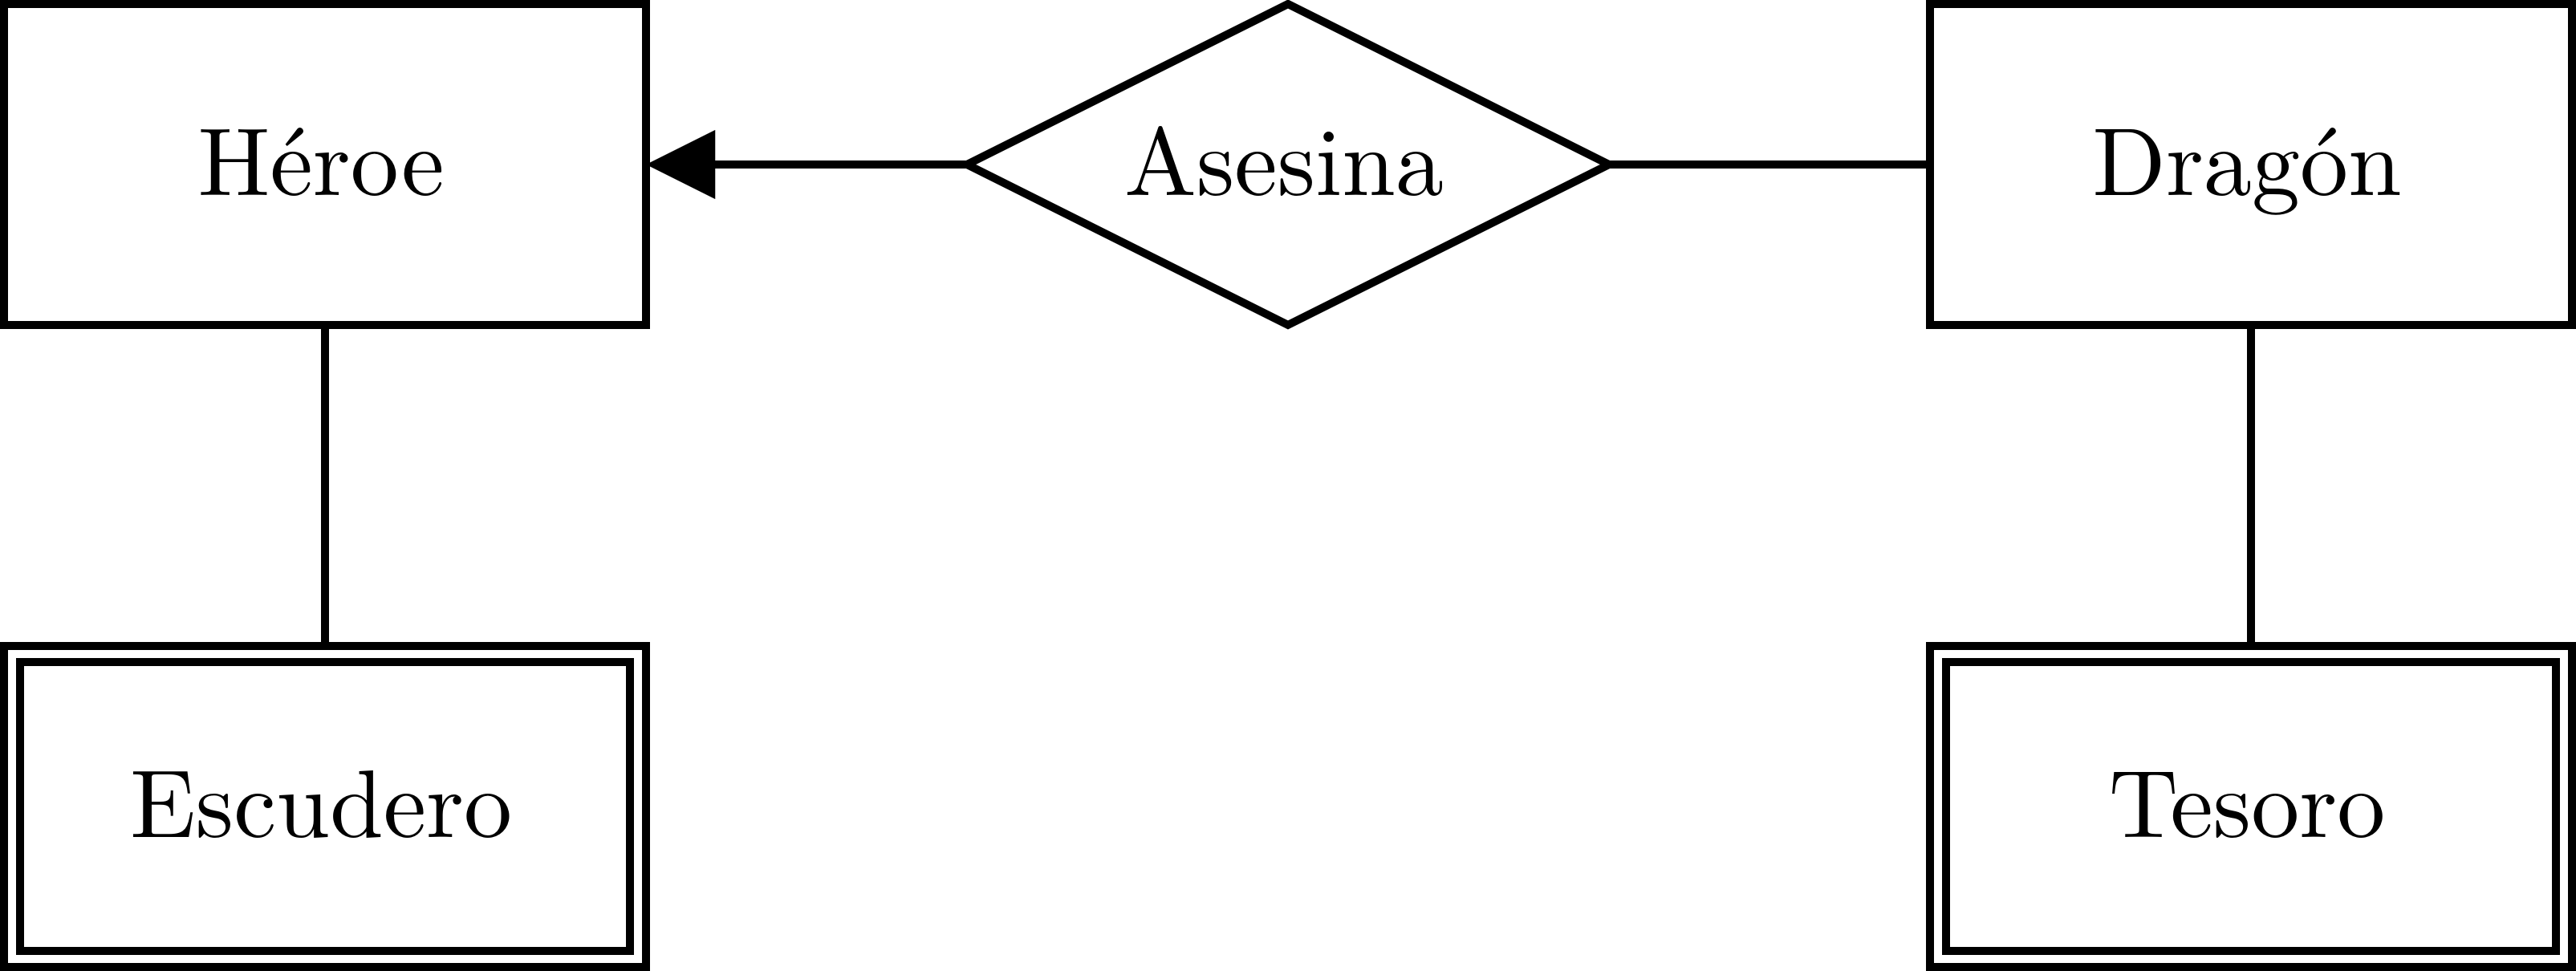
\includegraphics[scale=0.05]{HeroeAsesinaDragon}
\end{center}
\caption{Diagrama E/R en el que un héroe asesina muchos dragones}
\end{figure}

Marcamos la cardinalidad de las relaciones mediante la presencia o ausencia de punta en las líneas que unen las entidades con la relación.
Una línea sin punta indica que la entidad a la que apunta posee una cardinalidad de \textit{muchos} y una línea con punta, de \textit{uno}.

\begin{figure}[h]
\begin{center}
	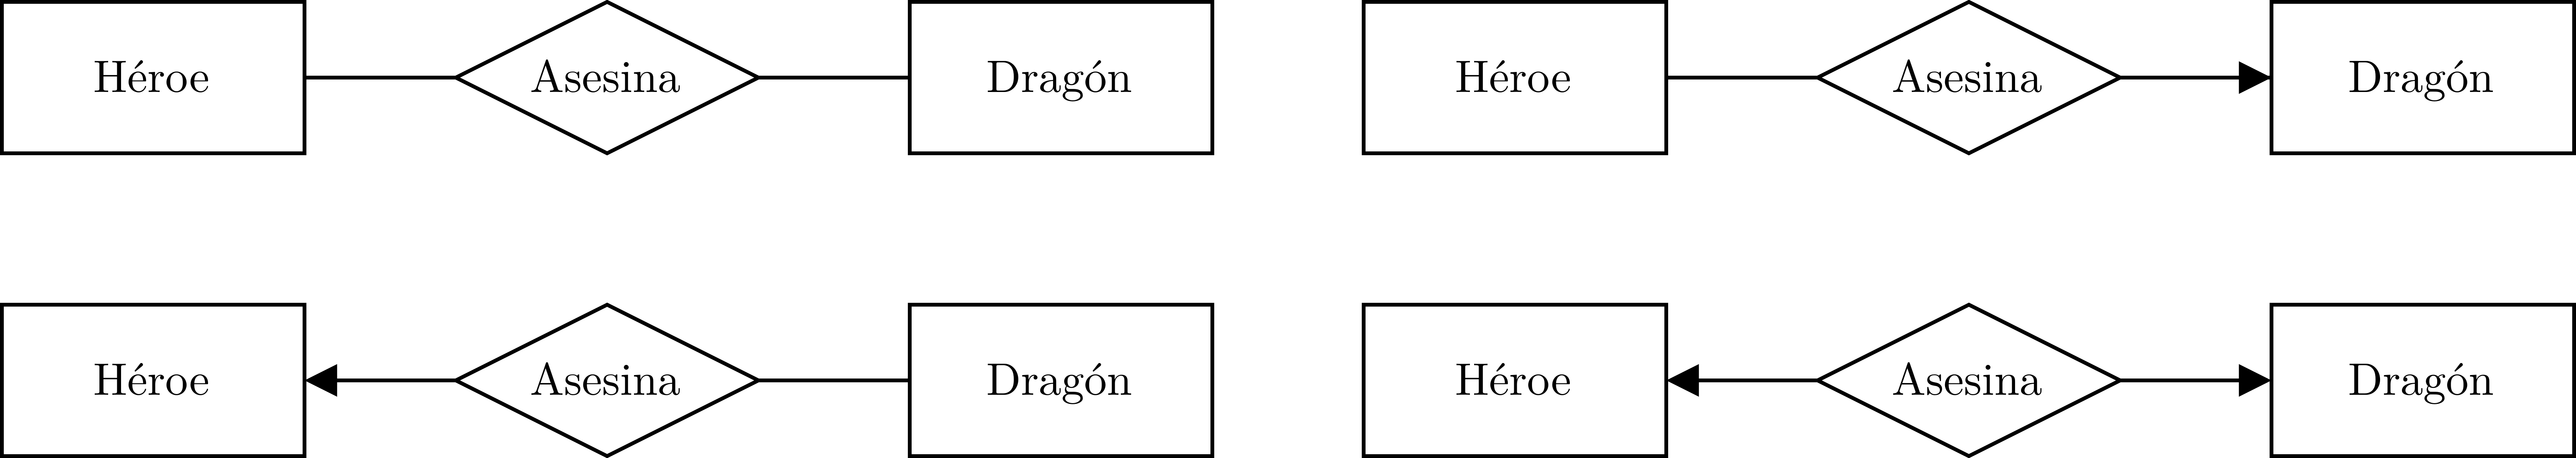
\includegraphics[scale=0.05]{Cardinalidades}
\end{center}
\caption{Relaciones \textit{muchos a muchos}, \textit{muchos a uno}, \textit{uno a muchos} y \textit{uno a uno}}
\end{figure}

Si una relación es de participación obligatoria lo marcamos con dos líneas paralelas para la parte restringida por esta obligatoriedad.
Por otro lado, si la relación es involutiva debemos especificar los roles junto a cada una de las líneas que unen la entidad con la relación.

\begin{figure}[h]
\begin{center}
	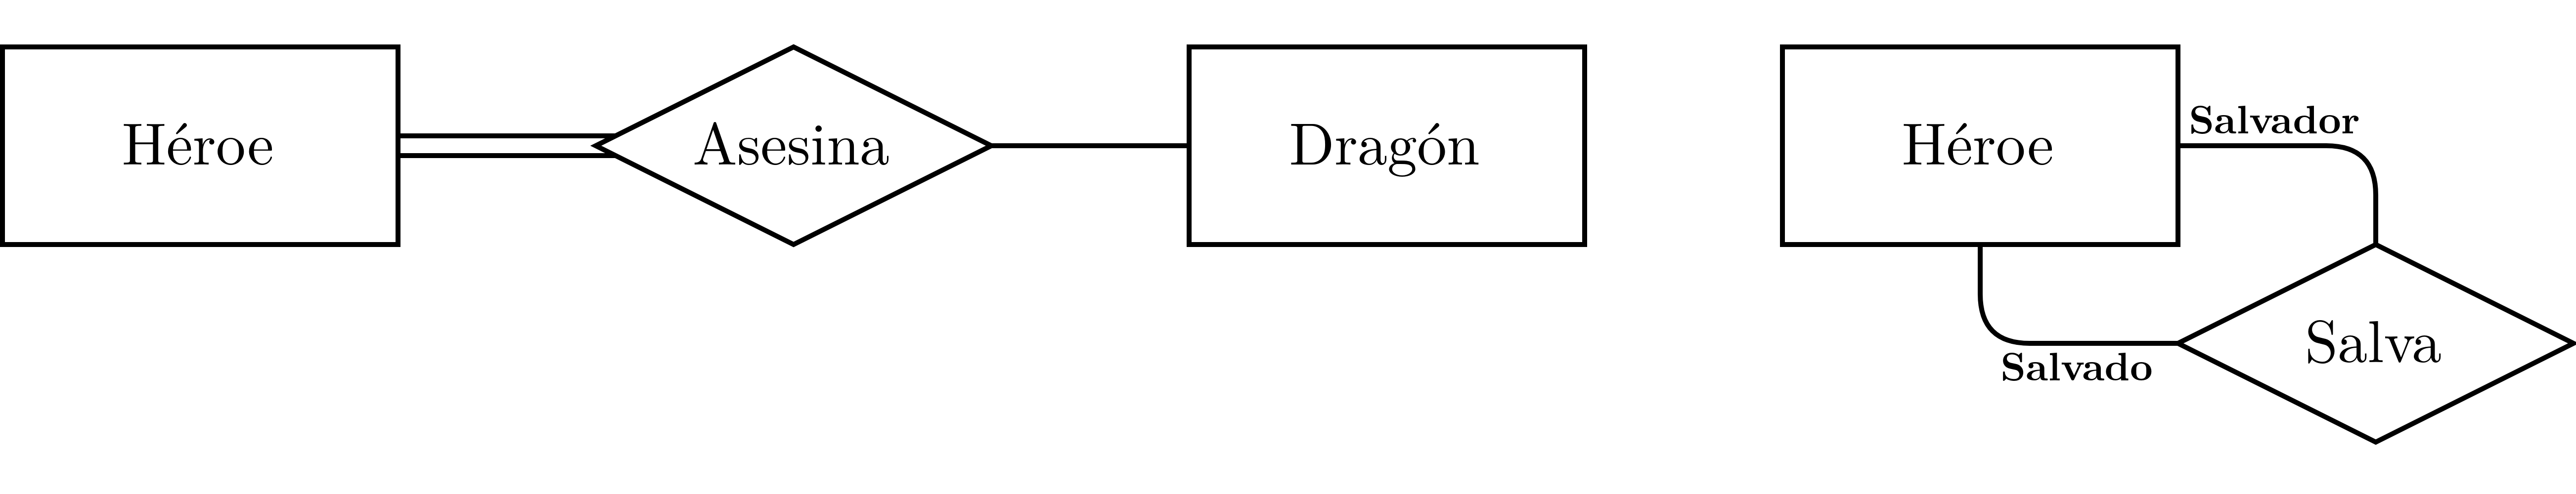
\includegraphics[scale=0.06]{ObligatoriaReflexiva}
\end{center}
\caption{Relaciones de participación obligatoria y reflexiva}
\end{figure}

Para indicar los atributos de las entidades y las relaciones utilizamos flecha acabadas en punta redonda que salen de éstas.
La forma de esta punta, la línea y el texto determinan el tipo de atributo:

\begin{itemize}
	\item\textbf{Punta vacía:} Atributo simple.
	\item\textbf{Punta vacía con nombre subrayado:} Atributo derivado o calculado.
	\item\textbf{Punta rellena:} Atributo con clave primaria o candidata
	\item\textbf{Punta rellena con línea discontinua:} Atributo discriminador o clave parcial en entidad débil o en relación.
	\item\textbf{Varias puntas rellenas atravesadas por una línea con punta rellena:} Clave primaria o candidata compuesta.
	\item\textbf{Varias puntas rellenas con líneqa discontinua atravesadas por una línea con punta rellena:} Atributo discriminador o clave parcial compuesta en entidad débil o relación.
\end{itemize}

\begin{figure}[h]
\begin{center}
	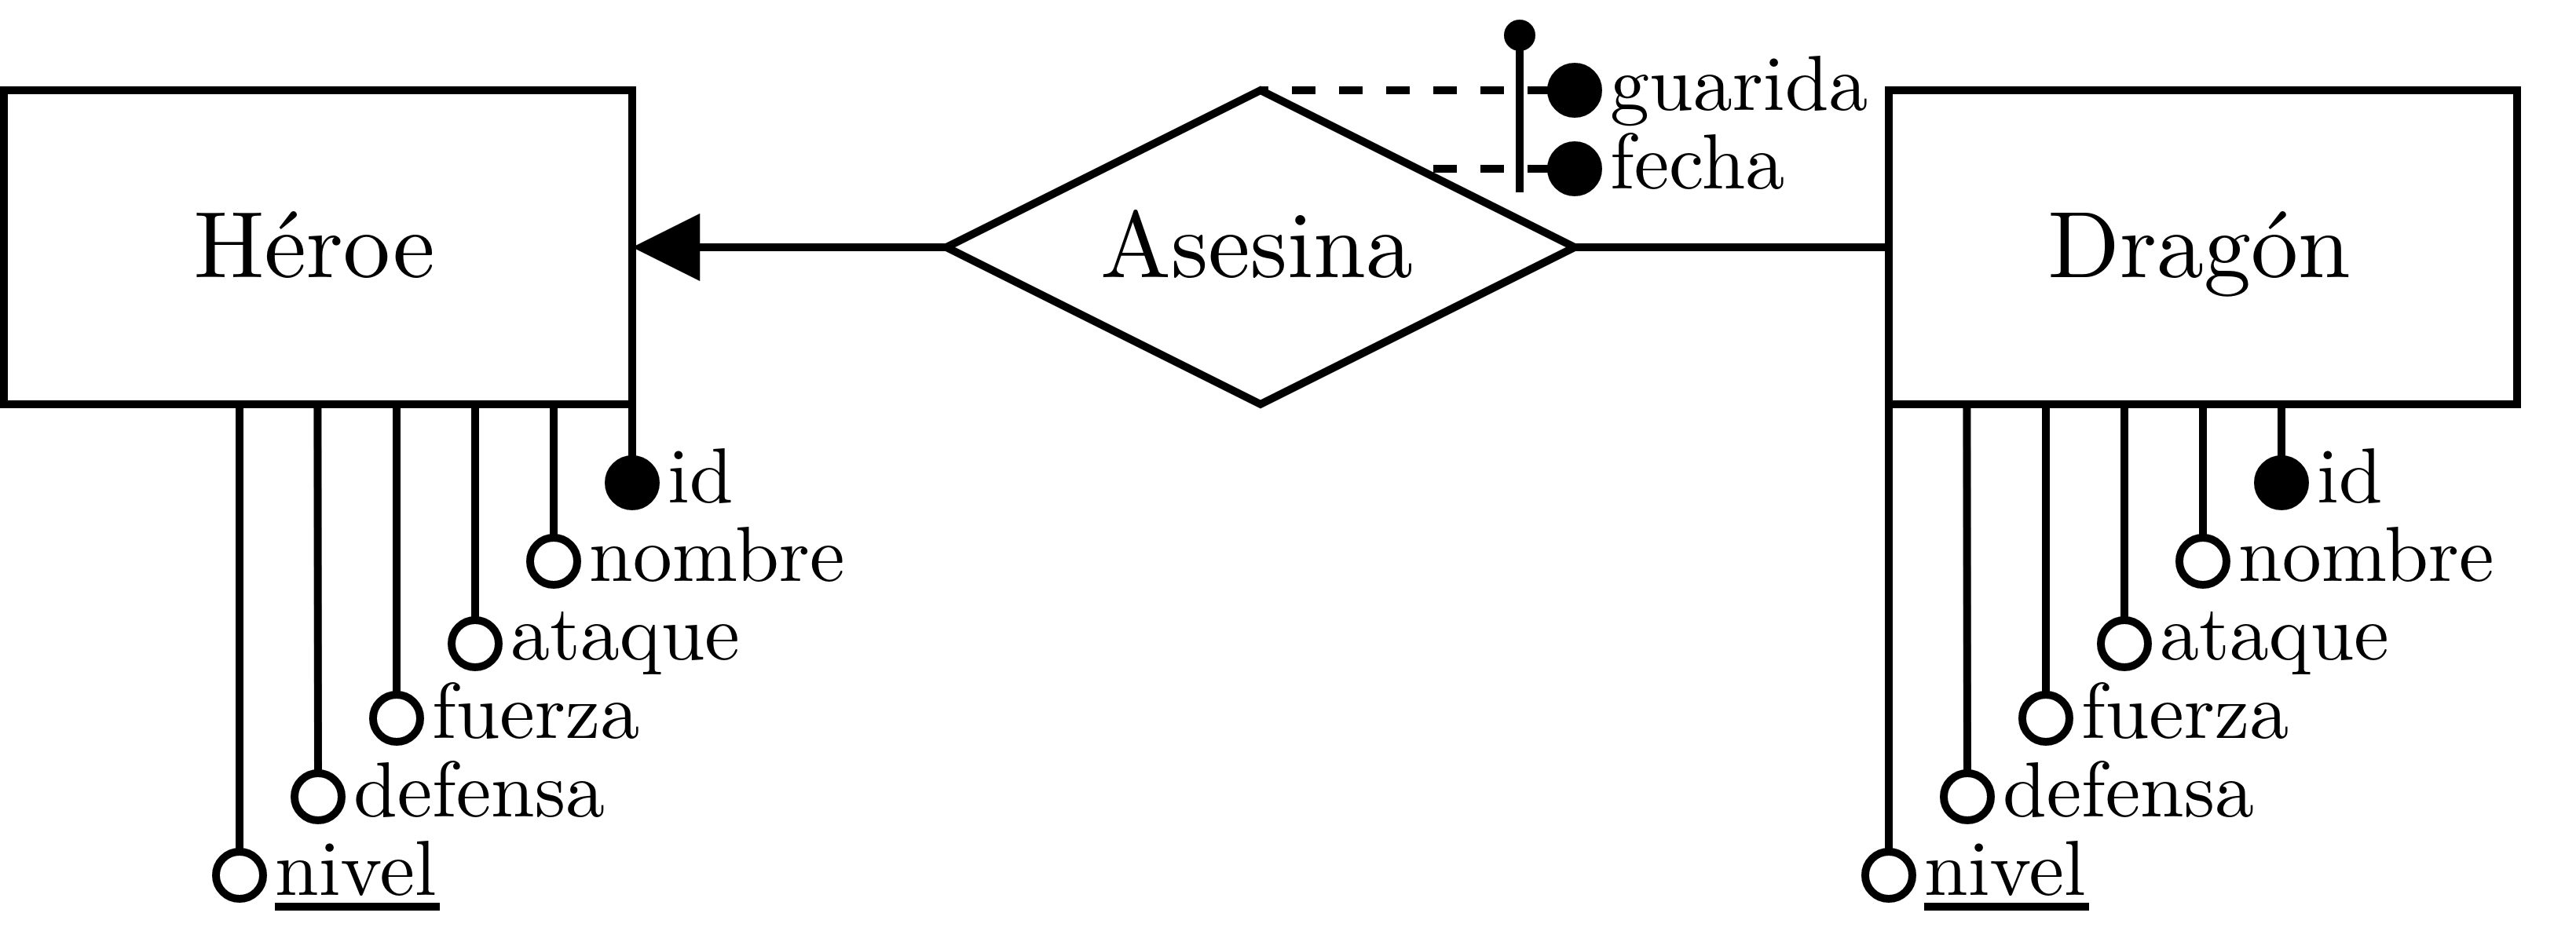
\includegraphics[scale=0.06]{Atributos}
\end{center}
\caption{Atributos simples, calculado, claves primarias y atributos discriminadores compuestos}
\end{figure}

Al especificar atributos discriminadores en las relaciones nos aseguramos de que siempre que se cree una instancia de la relación ésta debe unir necesariamente dos entidades y de que una instancia de una entidad $E_1$ no pueda relacionarse con otra entidad $E_2$ con el mismo atributo discriminador.
En el ejemplo de la figura anterior, un \code{héroe} no puede asesinar a más de un \code{dragón} en la misma \code{guarida} y en la misma \code{fecha}.

\section{Otros elementos del modelo E/R extendido}

El modelo E/R extendido (EE/R) permite más formas de relacionar y trabajar con las entidades de la BD\@.

\subsection{Herencia/especialización}

Sean dos conjuntos de entidades $A$ y $B$, definimos formalmente la especialización de la siguiente forma:

\[A\text{ es una especialización de }B\Leftrightarrow\forall a\in A\Rightarrow a\in B\]

Al igual que en la programación orientada a objetos, la relación de una entidad hija con una entidad ancestra es una relación de \textit{es un}, de forma que debemos poder afirmar que la clase hija \textit{es-un} padre (una \code{PSP} \textit{es una} \code{consola}).
En el diagrama E/R lo representamos con un triángulo invertido que contenga la expresión \code{es}, \code{es-un} o alguna variante de la misma.

Si la relación de herencia es \textbf{obligatoria}, es decir, no puede existir una instancia de la entidad padre sin ser una instancia de la entidad hija, lo indicamos con dos líneas paralelas que unen la base del triángulo y la entidad padre.
Si la relación de herencia es \textbf{exclusiva}, es decir, una entidad no puede ser de dos tipos a la vez, lo indicamos con la plabra \code{Disjunta}.
Las relaciones de herencia pueden ser obligatorias y exclusivas a la vez.

\begin{figure}[h]
\begin{center}
	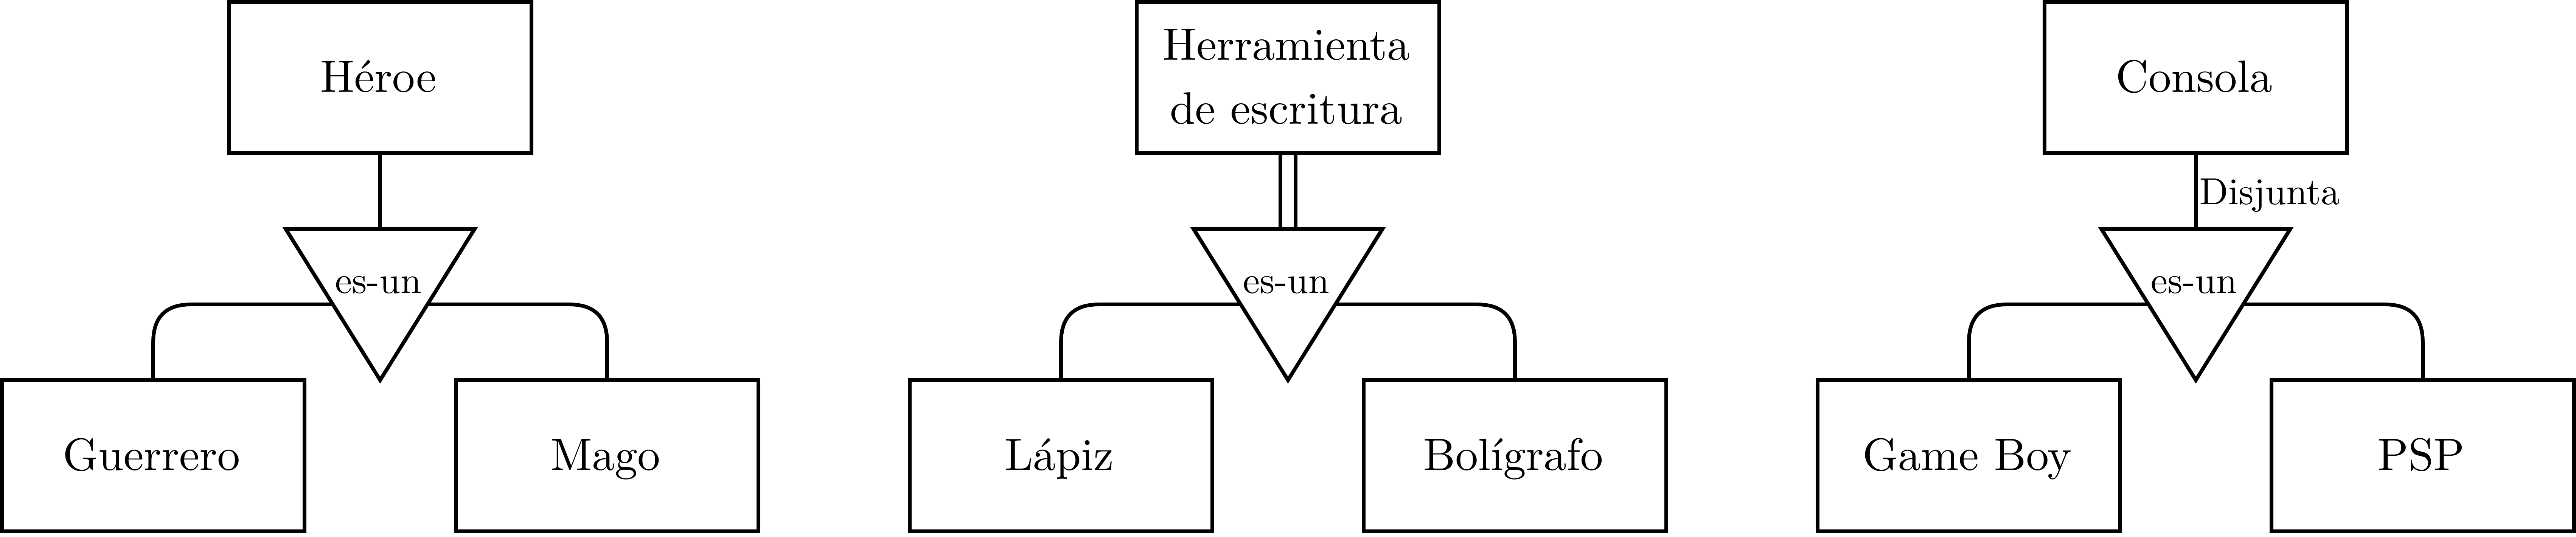
\includegraphics[scale=0.06]{Herencia}
\end{center}
\caption{Relación de herencia, de herencia obligatoria y de herencia exclusiva}
\end{figure}

De nuevo, al igual que en la programación orientada a objetos, las entidades hijas heredan automáticamente todos los atributos de sus entidades ancestras.

\subsection{Agregación}

Las agregaciones agrupaciones de entidades y relaciones que encapsulan varias entidades y sus relaciones en una entidad genérica que podemos referenciar sin especificar su estructura interna.
De ellas sólo necesitamos conocer las claves primarias para referenciarlas desde su exterior.

\begin{figure}[h]
\begin{center}
	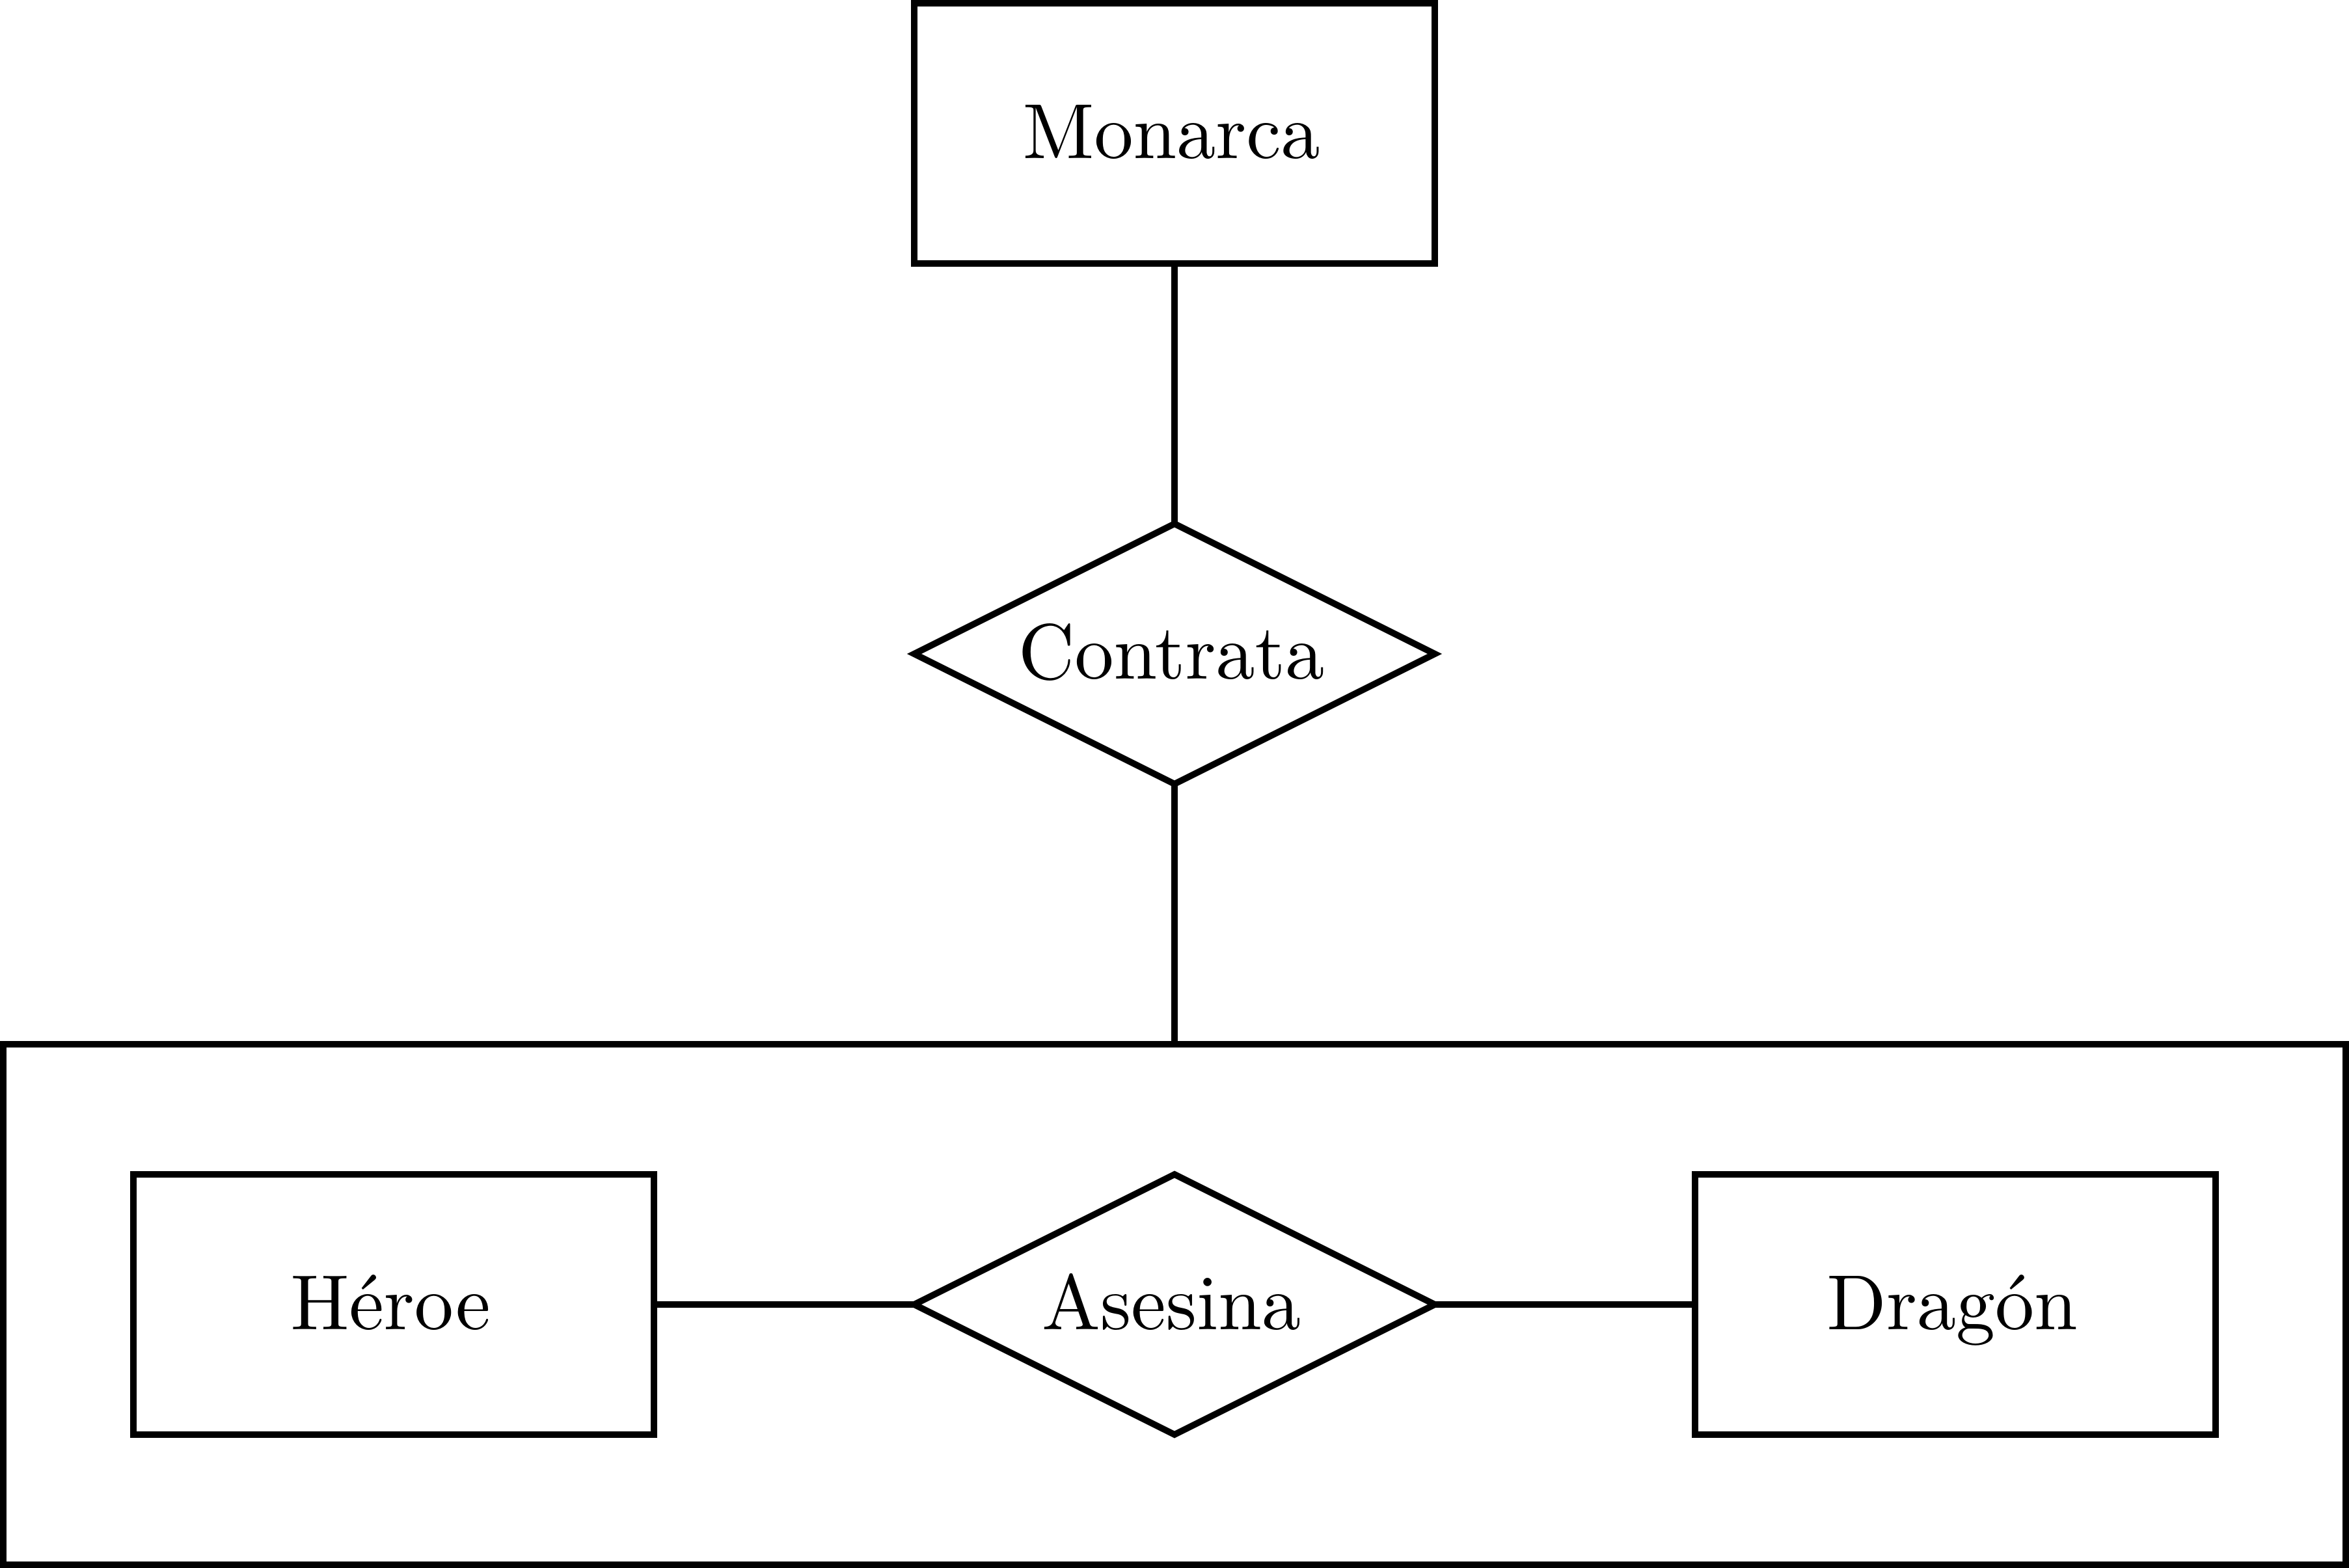
\includegraphics[scale=0.06]{Agregacion}
\end{center}
\caption{Relación de agregación sobre el contrato de asesinato de dragones}
\end{figure}

En la figura anterior podríamos haber tenido que un \code{Monarca} \code{contrata} a un \code{Héroe} y que la labor de este \code{Héroe} es \code{asesinar} a un \code{Dragón}.
Sin embargo, como en nuestro ejemplo los \code{Héroes} siempre \code{asesinan} \code{Dragones}, podemos encapsular el \code{contrato} en una agregación y referirnos a la relación entre el \code{Héroe} y el \code{Dragón} como una entidad propia.

\pagebreak

Debemos tener en cuenta que las relaciones no siempre tienen que ser binarias, sino que pueden ser ternarias, cuaternarias o de cualquier aridad.
Estos tipos de relaciones complican la estructura del diagrama y pueden presentar problemas de diseño, por lo que suele ser mejor utilizar agregaciones para simplificar la estructura y reducir la probabilidad de cometer errores.

\begin{figure}[h]
\begin{center}
	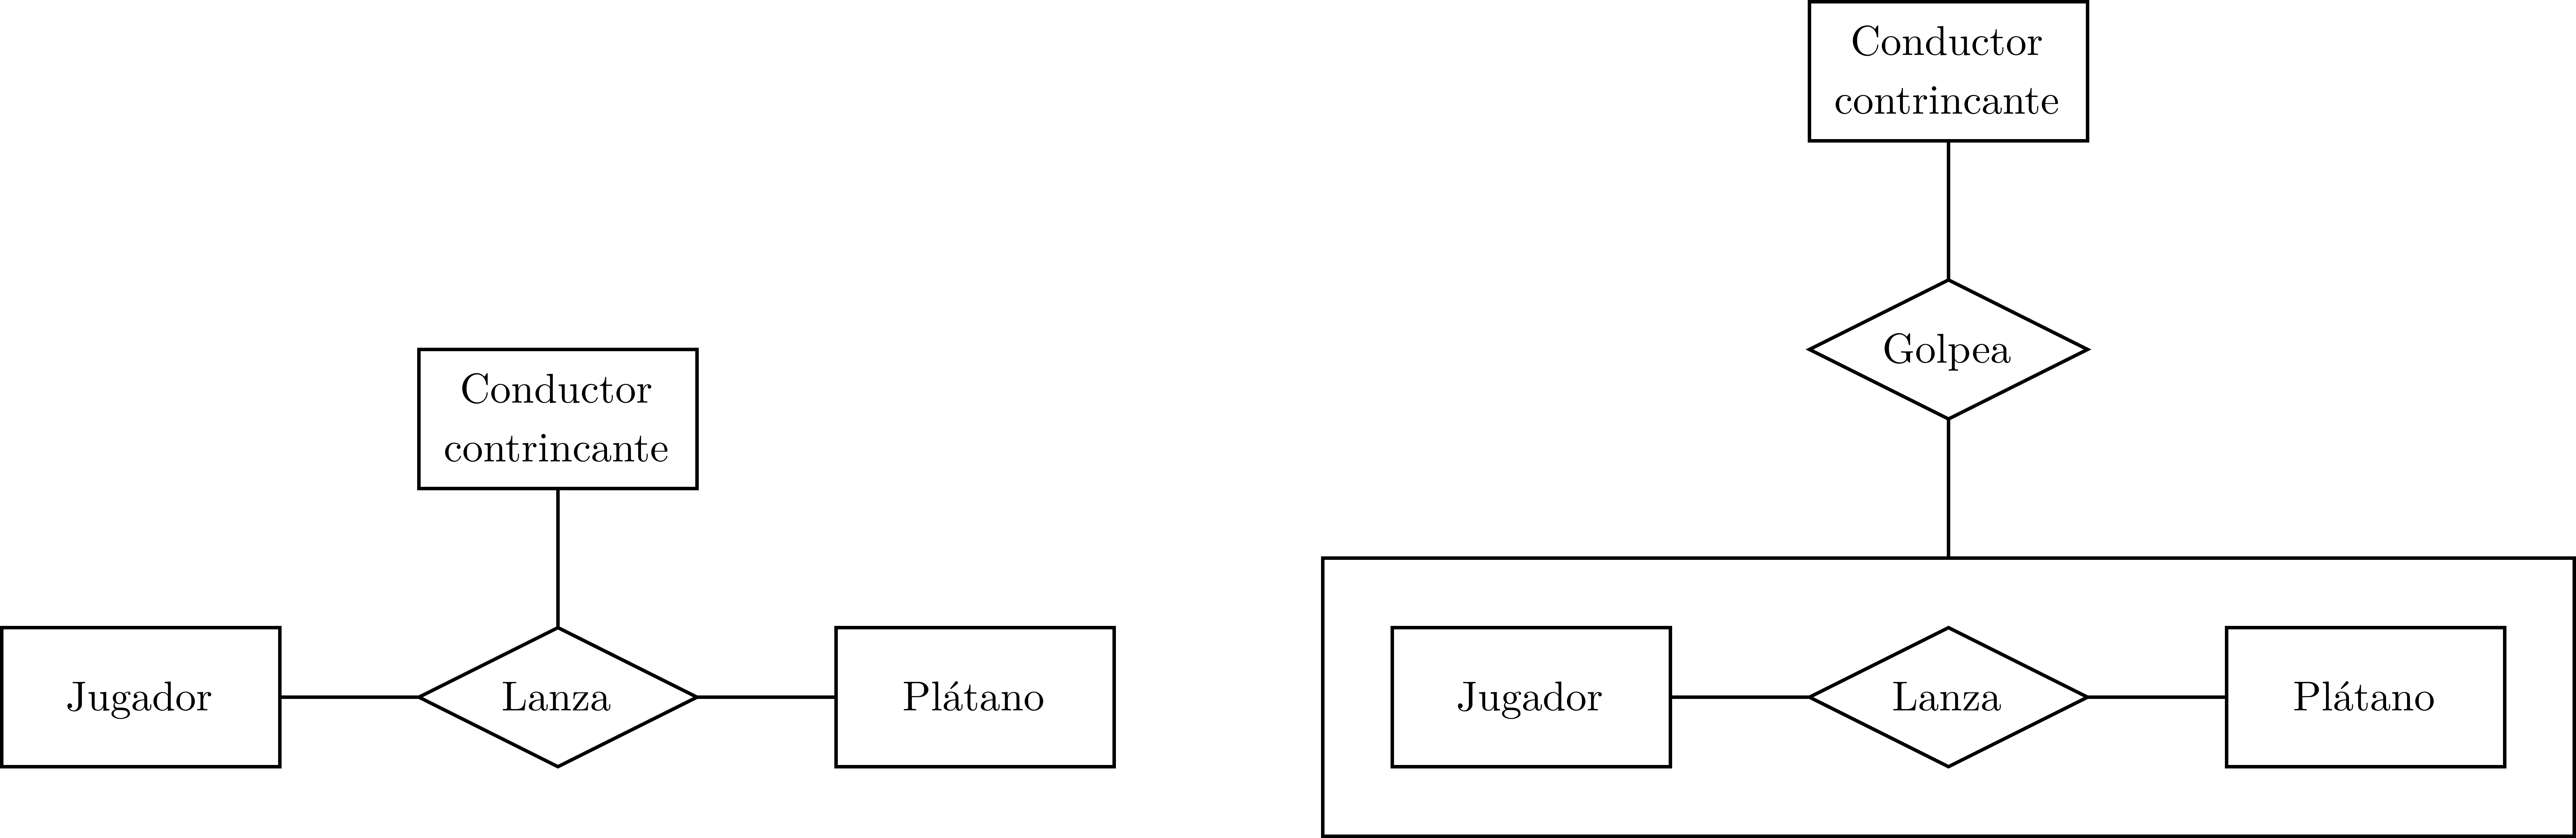
\includegraphics[scale=0.06]{TernariaVSAgregacion}
\end{center}
\caption{Relación ternaria en contraposición a una agregación}
\end{figure}

Sin embargo, las agregaciones no son soluciones a los ciclos de relaciones.
Aunque éstos pueden reflejar información redundante, las agregaciones eliminan información que en este caso es imprescindible.

\begin{figure}[h]
\begin{center}
	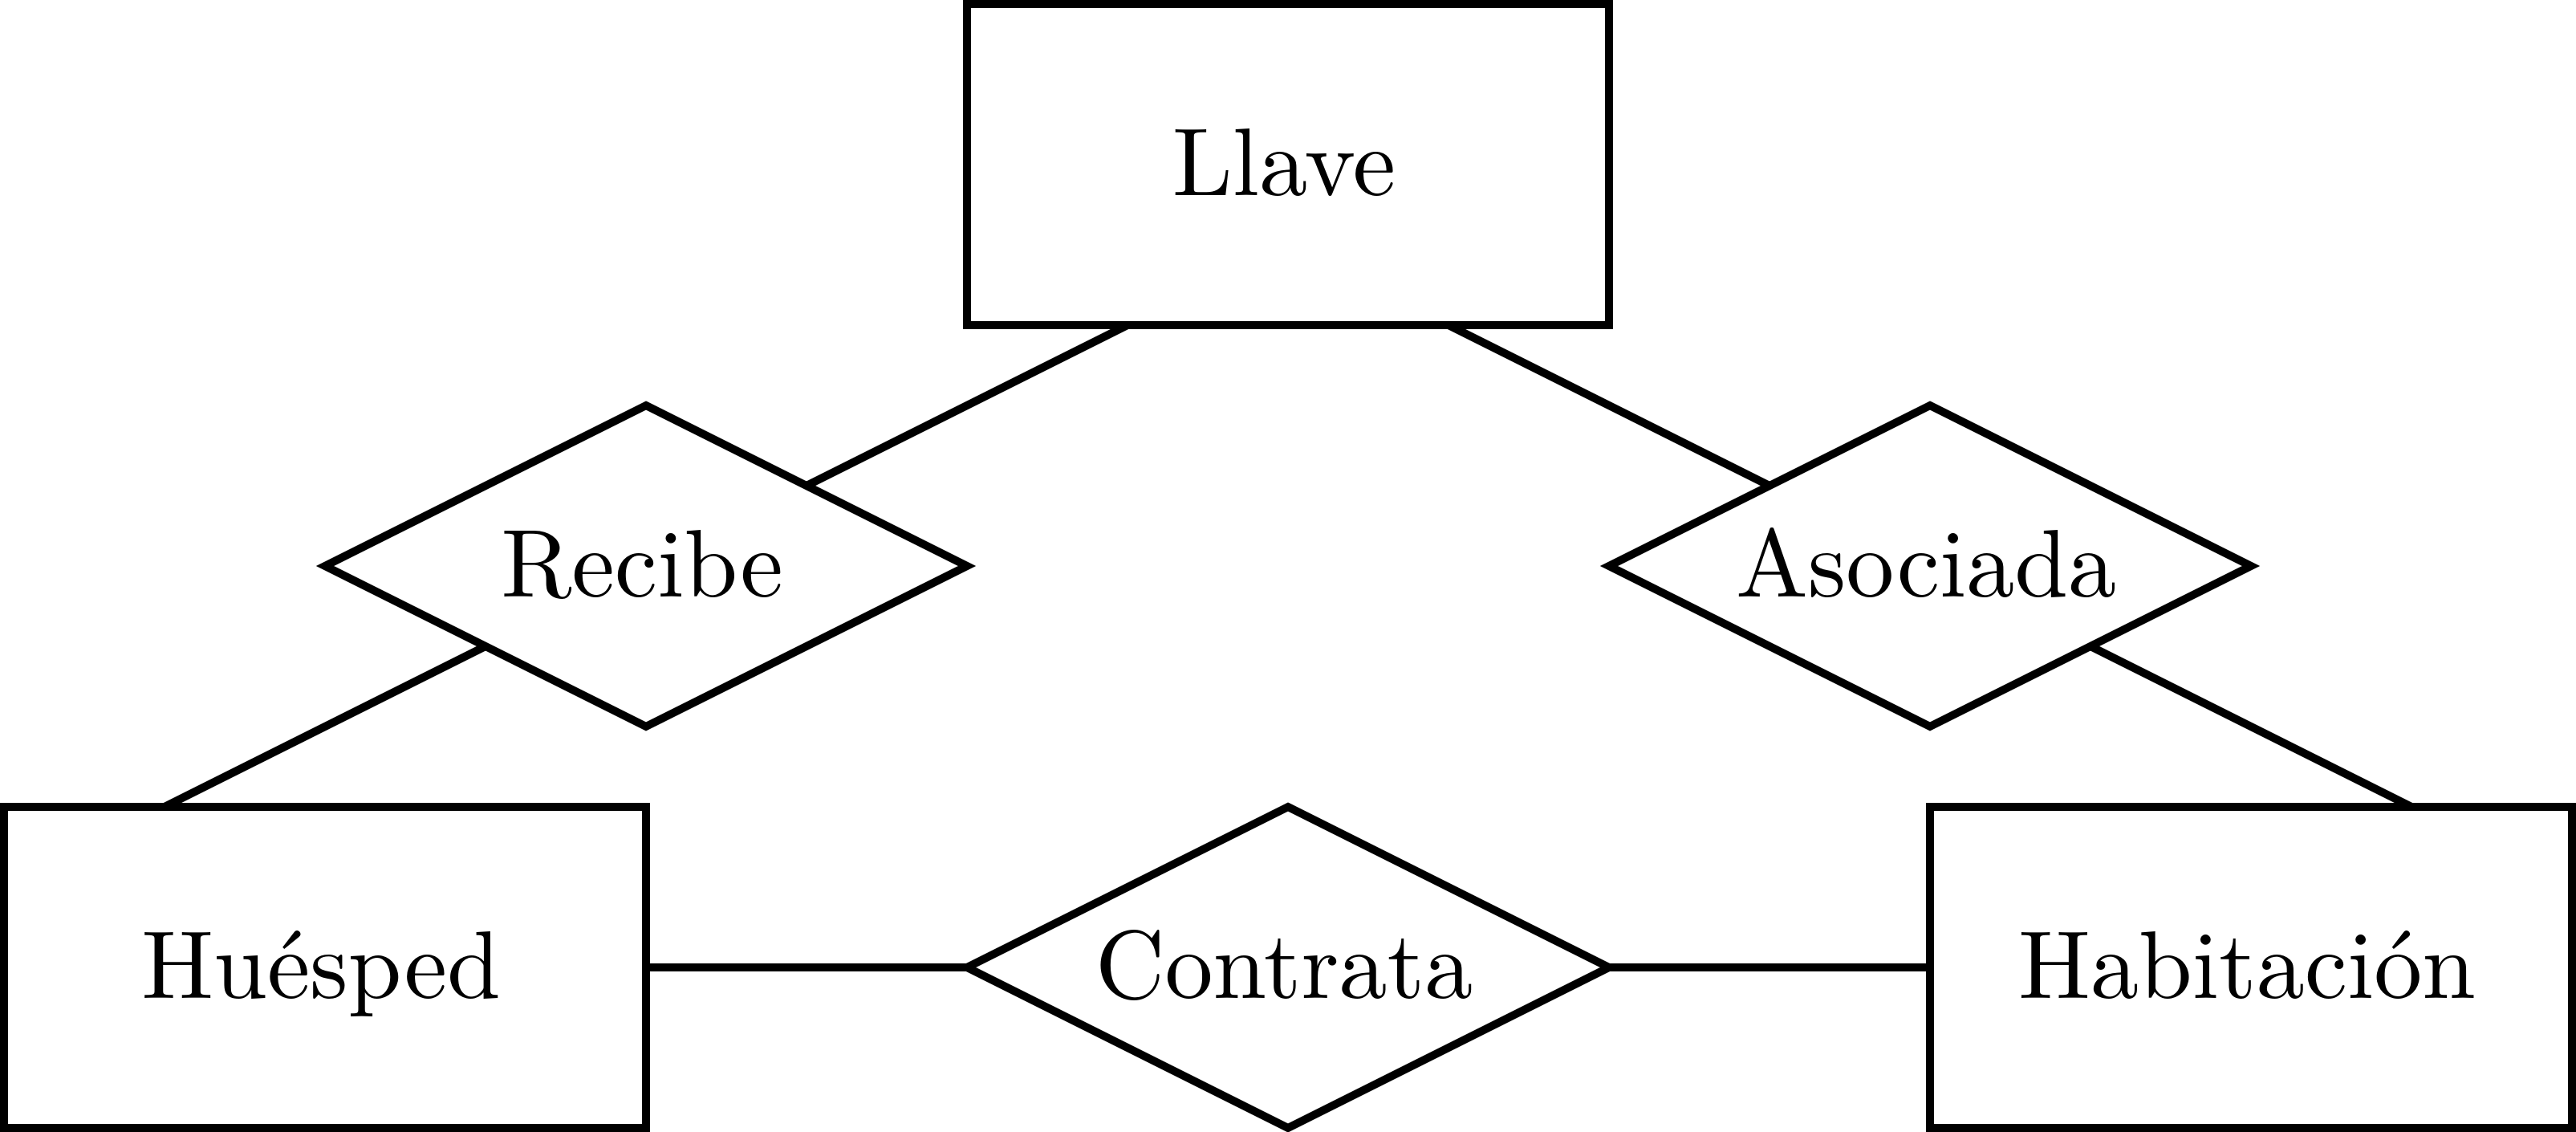
\includegraphics[scale=0.06]{Ciclo}
\end{center}
\caption{Ciclo de relaciones y entidades}
\end{figure}
